\documentclass[sigconf]{acmart}

\usepackage[english]{babel}
\usepackage{blindtext}
\usepackage{booktabs} % For formal tables
\usepackage{epsfig,endnotes,subcaption,url}
% Copyright
\renewcommand\footnotetextcopyrightpermission[1]{} % removes footnote with conference info
\setcopyright{none}
\settopmatter{printacmref=false, printccs=false, printfolios=true}

% DOI
\acmDOI{}

% ISBN
\acmISBN{}

%Conference
%\acmConference[Submitted for review to SIGCOMM]{}
%\acmYear{2018}
%\copyrightyear{}

%% {} with no args suppresses printing of the price
\acmPrice{}

\newcommand{\RF}[1]{{\bf\color{orange}(Romain) #1}}


\begin{document}
\acmConference[SIGMETRICS'20]{SIGMETRICS 2020}{June 2020}{XX, YY}
\title[Skylines]{Skylines: Demystifying Network Resource Islands with Virtual Landmarks}

%
% I use a file for every section.  Each of these corresponds to a file
% with the specified name ending in '.tex' (e.g., introduction.tex).
%

%   ==========================================================================
%   AUTHORS
%   ==========================================================================
%    \author{Marc Anthony Warrior}
\affiliation{%
  \institution{Northwestern University}
}
\email{warrior@u.northwestern.edu}
\author{Romain Fontugne}
\affiliation{%
  \institution{IIJ Innovation Institute}
}
\email{romain@iij.ad.jp}
\author{Randy Bush}
\email{randy@psg.com}

\renewcommand{\shortauthors}{M. Warrior et al.}

%\author{Paper \# XXX, XXX pages}
% \author{Firstname Lastname}
% \authornote{Note}
% \orcid{1234-5678-9012}
% \affiliation{%
%   \institution{Affiliation}
%   \streetaddress{Address}
%   \city{City} 
%   \state{State} 
%   \postcode{Zipcode}
% }
% \email{email@domain.com}


%   ==========================================================================
%   ABSTRACT
%   ==========================================================================
    \begin{abstract}

``Do you see what I see?'' The vastness of today's Internet creates an intuitive
but often overlooked phenomenon: not everyone is exposed to the same web
resources. Even across the set of objects embedded in a single web page, a pair of
clients with apparently similar network properties may be assigned to barely
overlapping sets of network resources to pull from. While the properties of
individual content distribution networks (CDNs) and the like are well explored,
there has been, until now, a lack of insight regarding the \emph{aggregate}
behavior of these many large networks co-existing.  

In this paper, we perform the first, deep analysis of cross-provider resource
allocation patterns and the resulting aggregate mapping of over 10,000 RIPE
Atlas clients around the world. To facilitate our research, we introduce common
network resource exposure (CNRE) - a measure of the degree to which a pair of
clients are exposed to the same network destinations as each other across a
large set of domains. We explore the implications of high and low CNRE scores,
and assess the applicability of well established network properties (country,
ASN, BGP prefix, and /24) in estimating CNRE. Our findings expose clients that
are poorly served by their current position in this aggregate mapping scheme and
highlight the existence of ``outlier'' CDNs, who allocate their resources in a
way that goes against broader Internet trends.

\end{abstract}



    \maketitle
%   ==========================================================================
    %   IMC generated code (document details)
%   ==========================================================================
    %
% The code below should be generated by the tool at
% http://dl.acm.org/ccs.cfm
% Please copy and paste the code instead of the example below. 
%

%   ==========================================================================
%   MAIN PAPER BODY
%   ==========================================================================
    \section{Introduction} \label{sect:intro}

You and the person next to you might not be using the same Internet. With
ever increasing diversity and interlinking of online services  --- content distribution networks (CDNs), cloud computing, CDN and
cloud brokers, ad brokers, load balancing, user tracking, geoIP, and more --- even the
implications
of loading a single web page are no longer straightforoard CITE. Often, failure to
recognize the whole as distinct from the sum of its parts has inhibited progress
and hampered performance in networking technology CITE. In the same way a city's
skyline cannot be anticipated by the artitect of a single  building, the
``digital skyline'' of the Internet can be neither predicted nor fully
controlled by any single entity.
However, skylines can always be \emph{observed}.

Even across a single network service, client experiences may diverge. In Figure
\ref{fig:dnsmiss}, we provide a high level illustration of how this can happen.
In subfigure \ref{fig:dns},  a client intending to connect to example.com submits a DNS query. We do not
concern the minute details of
the DNS resolution process, which is itself multi-tierd and possibly involving
cooperation from many separate stakeholders. What is important to know is that
eventually, the client's request reaches the nameserver responsible for
example.com. The nameserver uses what is often internal, proprietary
logic to decide which of example.com's network resources the client should be
connected to. In subfigure \ref{fig:mismatch}, we are reminded that this client
is not the only one access example.com. However, as illustrated,
the client's peers may not necessarily be directed to the same resource, despite
having carried out essentially the same DNS resolution process and possibly
sharing the same edge network. This potential for mismatch between clients only
grows as the number of domains considered increases --- which it will, often on
a single web page.

In this paper, we explore the complex combination of independently operating
resource allocation schemes and assess their behavior in \emph{aggregate}. To
enable our research, We introduce a new similarity measure, common network
resource exposure (CNRE), which captures the extent to which a pair of clients
are directed to the same network targets as each other across a broad set of
domains. CNRE is, to our knowledge, the first ever method to quantify
cross-provider DNS redirection patterns and their collective behavior. 

We test and assess CNRE using 302 web content hosting domains for each CNRE
calculation.  To do this, we collect latency and DNS measurements for each
domain from each of 9,024 globally distributed clients and perform over 40
million pairwise CNRE calculations between them. Our experiments 
validate common network research exposure as a useful quantity and explore its
relationship with other cilent properties.

\begin{figure*}
    \center
        \mbox{
            \begin{subfigure}[b]{0.5\linewidth}
                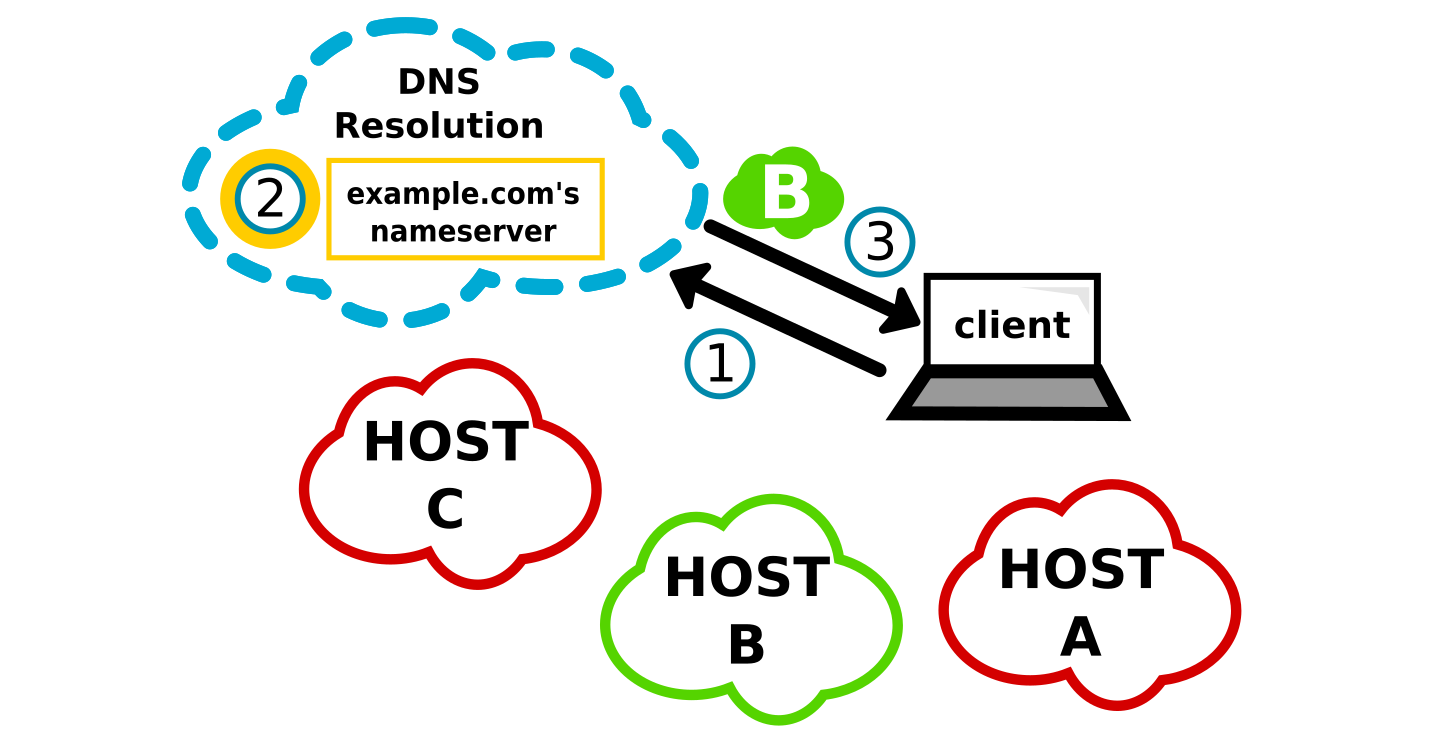
\epsfig{file=figs/dns_resolution.png, width=1\linewidth}
                \caption{\label{fig:dns}}
            \end{subfigure}
            \begin{subfigure}[b]{0.5\linewidth}
                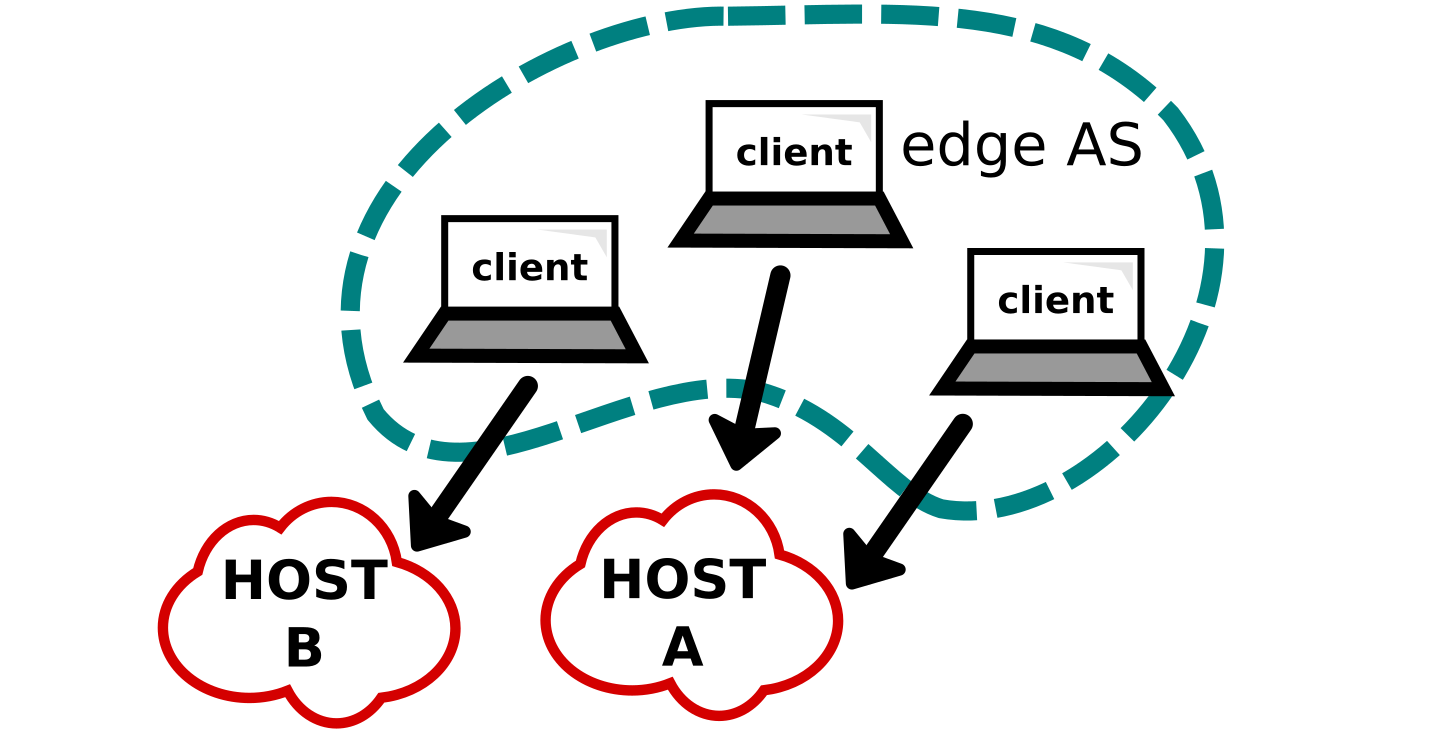
\epsfig{file=figs/client_mapping.png, width=1\linewidth}
                \caption{\label{fig:mismatch}}
            \end{subfigure}
        }
    \caption{
        Illustration of network resource allocation. Figure \ref{fig:dns} shows DNS resolution at a high level: 1)~The client deploys a DNS query for example.com. 2) This query ultimately reaches nameserver responsible for example.com and decides which of example.com's network resources should serve the client. 3) The nameserver's resource selection is returned to the client. Figure \ref{fig:mismatch} shows an example of how clients with similarly described locations may
        be directed to distinct network resources.
    }
    \ref{fig:dnsmiss}
\end{figure*}

In order to develop the Skyline model, we performed an exhaustive set of measurements to frame
client experience on a per \emph{site} basis. In this work, we capture a
snapshot of both DNS resolutions and latency measurements toward the 304 domains that appeared most
frequently in the top 2441 most popular webpages. Our measurements span over
9,000 unique
clients spread across 185 countries and 3637 autonomous systems. We performed over 52 million pairwise
comparisons with the results of these measurements to arrive at the foundation of what we have
coined the ``Skyline model". 

This paper makes the following contributions: %, including those we expect to stem from
%proposed work, which we have designated with (\emph{p})

\begin{itemize}%\parskip0pt \parsep0pt
    \item We perform a large exploration of client network performance on a per webpage level. Our
        raw results are publicly available on the RIPE Atlas platform.
    \item  We quantify the degree of misalignment between conventional grouping schemes
        and aggregate catchments.
    \item  We introduce the Skyline model, a client grouping scheme that reflects the
        extent of CNRE.
    \item  Using the Skyline model, we identify and analyze network resource islands --- 
        sets of clients with very high degrees CNRE. 
\end{itemize}

% RELATED WORK and PROBLEM FRAMING
\section{Problem Space and Related Work} \label{skyspace}

This projects aims to gain an understanding of which clients are directed to the same set of
resources across many distinct domains. Its most direct and immediate use case is influencing probe
selection in large scale Internet measurements. For researchers, likely unaware of the relatively
hidden allocation schemes of the wide array of CDN platforms and other large content distributors,
it is difficult to determine, a priori, the degree of similarity between clients. Knowledge of
whether there is a high probability that a pair of clients are being directed to altogether
different resources may be significant to their experiment design. This approach to experiment
design is in line with RIPE Atlas, one of the largest client based measurement platforms,
which maintains
an exhaustive set of tags on all of their clients in order to help researchers and network operators
filter and refine the set selected for their experiment \cite{ripe-atlas}. Further, more abstract
applications may include, but are not limited to, distributed denial of service mitigation
\cite{anycastvsddos} and CDN node deployment \cite{35590, Tariq}.

The most similar body of related work involves anycast CDN catchment analysis, which aims to
investigate the set of clients routed towards particular CDN points of presence (PoPs)
\cite{Calder2015, anycastvsddos, vdmscatchment}. Our work differs significantly in scope: to our 
knowledge, we are the first to investigate what we refer to as \emph{aggregate catchments}, the joint
behavior of many anycast CDN catchments and unicast CDN targets, spread across many content
distribution platforms. Conversely, this related body work either focuses on individual platforms or
specific services \cite{Calder2015, anycastvsddos, vdmscatchment}. 

Several authors have attempted to discover the topology of large CDN platforms through large scale
measurement studies \cite{webcart, Calder2013, benson11}. While their findings are potentially of
use in this project, their goals and contributions run parallel to what we aim to accomplish. They
seek to identify the properties and locations of CDN resources; conversely, we seek to identify the
target pools (sets of clients) of overlapping CDN resource catchments \cite{webcart, Calder2013,
benson11}. Other work close to this space investigates the performance of a particular CDN
deployment scheme \cite{ecs15sigcomm}.

    \section{Experiment \& Data Collection} \label{oversky}

The main preliminary steps performed to enable our
work are twofold: 1) domain name collection and 2) per-provider performance
measurement. The
remainder of this section details these steps and the reasoning behind them
while providing context with which to view results presented throughout this paper. 

\begin{figure}
    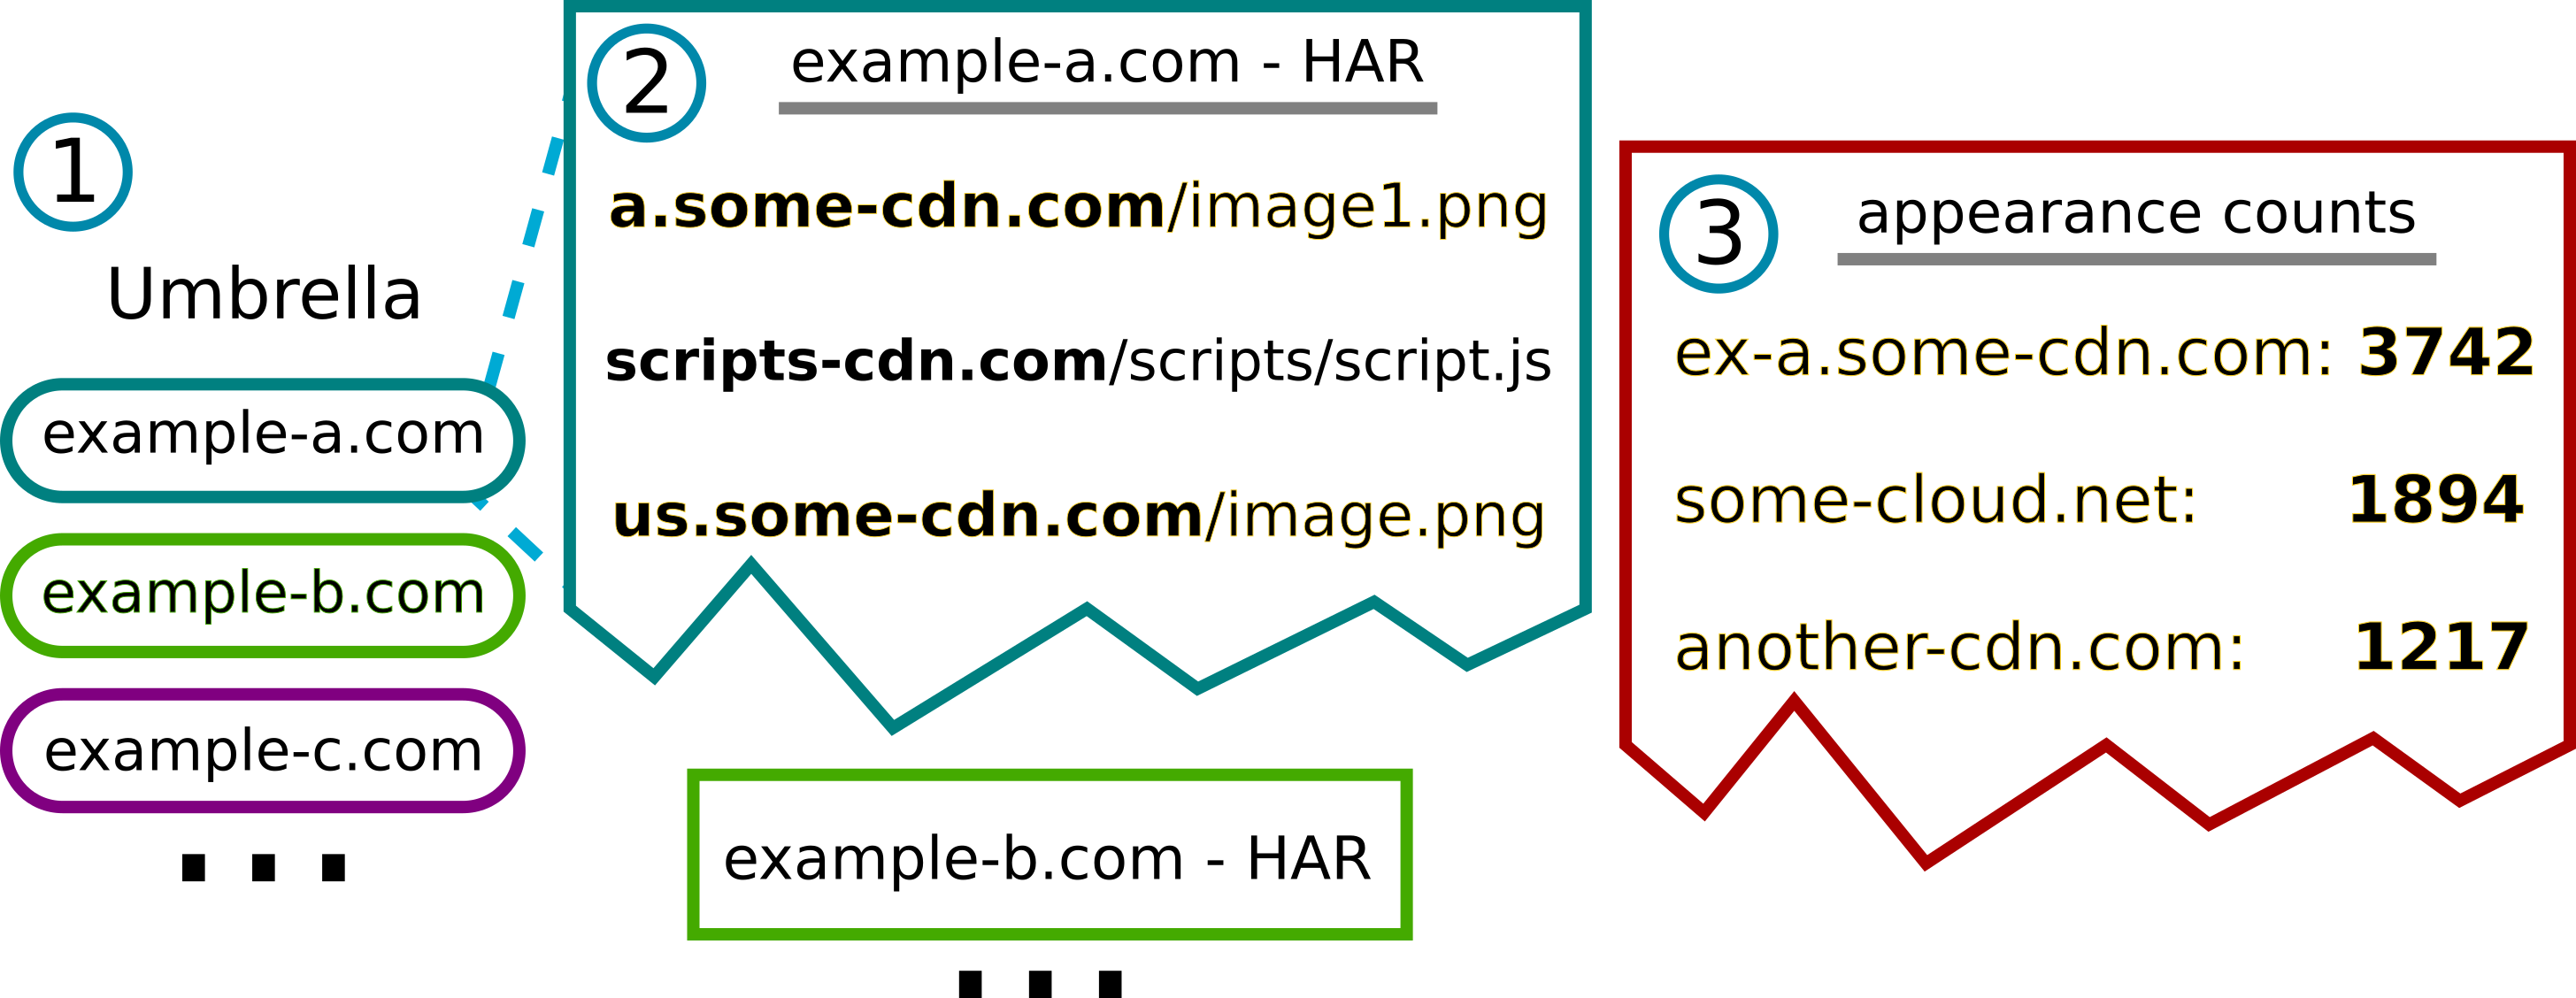
\epsfig{file=figs/domain_finding.png, width=1\linewidth}
    \caption{Diagram illustrating domain name collection: 1) Domains from the Umbrella top 1-million were loaded via Google Chrome to identify human-targeted websites. 2) For each human-targeted website's landing page, a HAR file was recorded. 3) Domains were extracted from HAR data and ranked by the number of times observed.
    }
    \label{fig:domfind}
\end{figure}

\subsection{Definitions}

As our aim in this paper is to explore the cross-provider behavior of Internet
resource-to-client mapping schemes, it is necessary to first establish what
qualifies as ``cross-provider'' and what sort of cross-provider behavior is of
relevance. For example, the reader may have observed that, if a pair of
providers are not used in \emph{together} for a given online experience, there
is no reason not to keep their analyses separate. For the purposes of this
paper, we choose to focus on the providers of webpage objects, which are known
to often span a multitude of providers CITE. Previous work has well documented
the impact of individual, slow loading objects on page load time CITE. To this
end, we target domains which we empirically found to co-inhabit large numbers of
webpages as web object hosts. Throughout this paper, we equate ``domain'' to
``host'' or ``provider'', recognizing, however, that it is often the case that a
single provider will use several domain aliases. 

Likewise, we also note here that our use of the term ``[web] resource'' is
deliberately ambiguous: the explicit implementation method used by each provider
--- ranging from a single subnet per geographic point-of-presence to a number of
software-partitioned subnets per machine --- is opaque and beyond the scope of
this paper. Our chief concern is that an identifiable distinction is made
between the set of targets (IP addresses) provided in DNS answers: the sheer fact that they are not
labeled as \emph{same} target indicates that there is likely some difference,
performance or otherwise, between them. For simplicity, we treat
each /24 IPv4 subnet (generally, the most fine-grained BGP prefix route
announcement allowed, by convention) as a potentially distinct resource, noting
that it may be the case that larger providers operate with smaller (more coarse
grained) prefixes.

\subsection{Domain Collection}

We use the top 10,000 most frequently resolved domains from Cisco's Umbrella Top
1-Million list CITE as a starting point. However, as this list is obtained from
the perspective of DNS resolution, the relationship \emph{between} these domains
is unclear. Further, as there is no complete URL information from such a
perspective, there is no indication which domains are used for downloading web
content, as opposed to providing some other service or interface. To address
this, we attempt to load pages from this list and ultimately use domains
providing web objects discovered on each successfully loaded page. This process
is detailed below and illustrated in Figure \ref{fig:domfind}.

First we attempt to load each web page from the Umbrella list using Google
Chrome. If a page loaded, its source was checked for any indication that the
page was not intended for human use (for example, automated server response
pages for non-200 HTTP status messages). This filter reduced the size of our
domain set from 10,000 pages to 2,441 pages. For each of these pages, a HAR file
(in HTTP Archive foromat file) was saved to capture the full set of web objects
loaded with the page. By using HAR files instead of just the page source, we
avoid missing any dynamically loaded objects that may not appear in the original
source. Even after using this approach, the space of possible domains remains larger
than we can address in the scope of this experiment. The HAR file provides the
full HTTP path of each web object retrieved. Domains used in this experiment
come from this dataset. 

Due to security related rate limits, our our experiment was limited to 15-20 domain measurements per
client per day, thus further restricting the number of domains to be used in our
experiment. Since the entire set obtained was large, we \emph{ranked}
object hosting domains by how frequently they wre observed across our set of HAR
files. The most frequently appearing object hosting domains were given priority.
Ultimately, 304 domains were used for the work described in this paper. 

\begin{figure}
    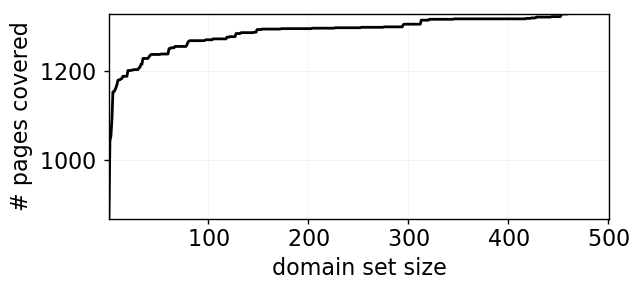
\epsfig{file=figs/num_sites_covered_by_top_n_doms.png, width=1\linewidth}
    \caption{The number of sites containing an object hosted by a domain in our set vs
    the size of our set of domains.}
    \label{fig:sitescovered}
\end{figure}

\begin{figure}
    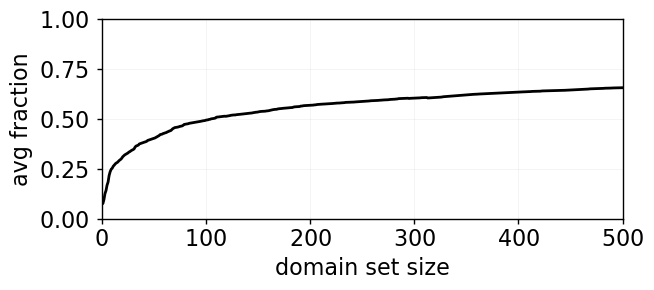
\epsfig{file=figs/fraction_links_covered_by_top_n_doms.png, width=1\linewidth}
    \caption{Mean fraction of page object links (URLs) covered per site vs the
    number of domains used.
    }
    \label{fig:linkscovered}
\end{figure}

In Figues \ref{fig:sitescovered} and \ref{fig:linkscovered}, we show the
decreasing marginal impact of each additional domain our set. As shown, both
quantities --- the number of visited pages including a URL from our domain set and the
fraction of URLs on each page addressed by our set --- exhibit logarithmic-like
growth patterns, beginning to plateau well before 100 domains are reached. We
assert that this demonstrates the aggregate behavior of the 304 domains obtained above
should sufficiently cover the domain diversity of a ``typical'' popular web page. 

\subsection{Per-Provider Performance Measurement}

Any attempt to identify the general groups that Internet clients are mapped to
requires a dataset with a uniquely broad scope: not only breadth --- a diverse
set of clients --- but also depth --- many clients from each, yet to be
uncovered, group or cluster. In addition, we are required to minimize the
temporal spread of the measurements, as network resource allocation is known to
change over time. We utilize the RIPE Atlas platform CITE for our measurements.
RIPE Atlas offers a large number of globally distributed clients, capable of
performing lightweight network measurements, such as pings, on behalf of
configurable requests received by the Atlas API. We deployed ping measurements
to the previously described 304 domains from 10,274 of RIPE's clients. Each
client performed DNS resolution for pings via their local DNS resolver, ensuring
that they each targeted the web resource they would ordinarily be directed to.

Unavoiable flux in the availability of individual, voluntarily maintained
clients lead to some clients to performinging only a subset of the given
measurements, thus missing some of the domains of interest. To be sure that this
does not dramatically affect our findings, we arbitrarily enforce minimal amount
of domain coverage --- 160 domains, just more than half of our set --- for use
of a given client's data. We show in Section REF the effects of domain quantity
in our measurements.

    \section{Common Network Resource Exposure} \label{sect:crne}

\begin{figure}
    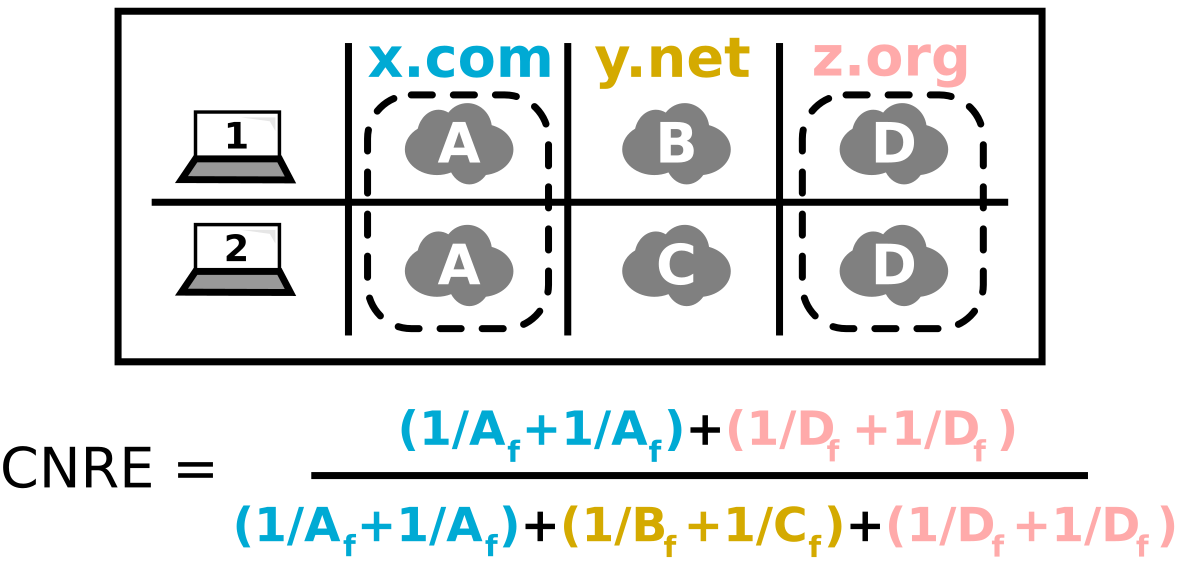
\epsfig{file=figs/cnre.png, width=1\linewidth}
    \caption{diagram illustrating CRNE}
\end{figure}

\begin{figure}
    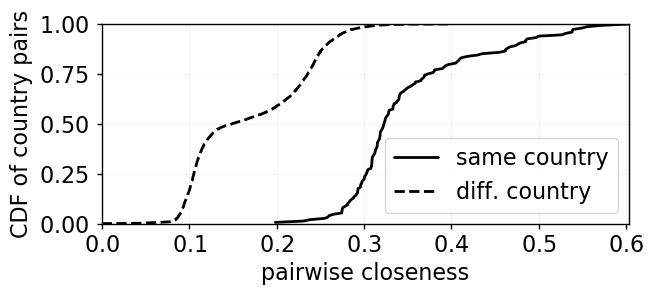
\epsfig{file=figs/country_cdf.png, width=1\linewidth}
    \caption{“High” closeness (90th percentile?) vs \# domains measured}
\end{figure}

\begin{figure}
    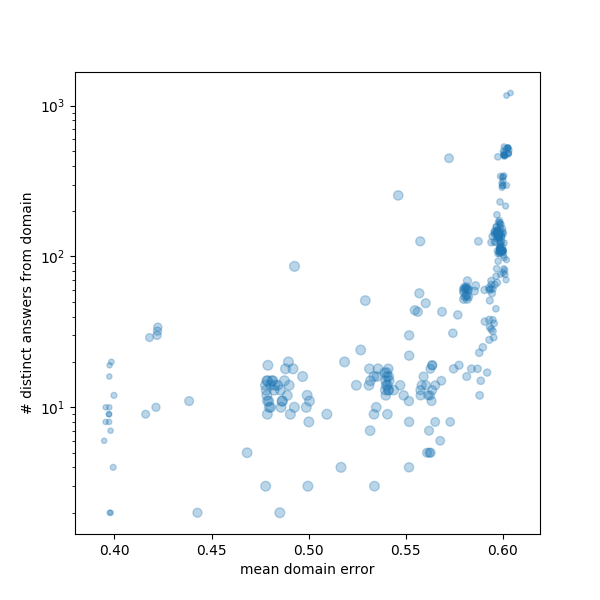
\epsfig{file=figs/domain_error.png, width=1\linewidth}
    \caption{Mean CNRE error vs \# of distinct answers observed from domain (one dot per domain). TODO: correct axis labels}
\end{figure}

    \section{Finding High CNRE Clusters} \label{sect:finding}

\begin{figure*}
    \epsfig{file=figs/dendrograms/v1.png, width=1\linewidth}
    \caption{Dendrogram of CNRE distance across all client pairs}
    \label{fig:dendrogram}
\end{figure*}

Finding aggregate catchments --- pools of clients essentially directed toward
the same web resources --- necessarily involves finding sets of clients with high
CNRE measures between each other. Because CNRE is a measure of similarity, this
problem naturally lends itself to hierarchical clustering techniques \cite{murtagh1983survey}. 
We employ the complete linkage method to ensure cluster formation reflects commonalities
across all cluster members as opposed to potentially edge-specific properties.
Note that in all \emph{clustering} calculations, we opt to use the CNRE \emph{distance}
(\(1-\)CNRE) as defined in Section \ref{sect:cnre}.

Establishing hierarchical clusters requires that we have some definition of what
constitutes a \emph{high} or \emph{low} CNRE measure and at what threshold it is
appropriate to consider clients sufficiently similar such that they appear in
the same cluster. In this section, we explore the implications of various CNRE
values, as well as CNRE's relationship with other, well-established client grouping
systems: country, ASN, BGP prefix, and /24 prefix subnet.

\subsection{Group Formation Patterns}
\label{s:formation}

Figure \ref{fig:dendrogram} presents a dendrogram derived from pairwise CNRE
distances across all clients and highlights two levels of distinct behavior
regarding the distribution of CNRE distances. In the uppermost portion of
the plot --- where CNRE distances are beyond a threshold of 0.65 --- we see
that distinctions between branches and their implied client groups become well
defined. 
There is a large cluster composed mainly of European and African probes (green 
cluster labelled \emph{Europe 95\%}), one representing East Europe (red cluster 
labelled \emph{DE 56\%}), one composed of North and South American probes (blue
cluster labelled \emph{US 59\%}), a cluster composed of probes from Asia
and Oceania (khaki cluster), and one made exclusively with American probes
(black cluster labelled \emph{North America 98\%}).
In the lower region of the tree, where CNRE distances drop below 0.65, we see 
that branches begin to fork unpredictably with shorter changes in CNRE distance. 
Some of these branches may map to specific countries, but at finer granularities
the geographical location of probes delineate poorly the characteristics
of the clusters.
%we mainly observe clusters with weaker correlations to the probe locations.
%Finally, in the lowest region of the plot, where CNRE
%distances drop below 0.25, we see the amount of branching increase once again,
%rapidly increasing the granularity of each branch as CNRE decreases further. 


\begin{figure*}
    \center
        \mbox{
            \begin{subfigure}[b]{0.33\linewidth}
                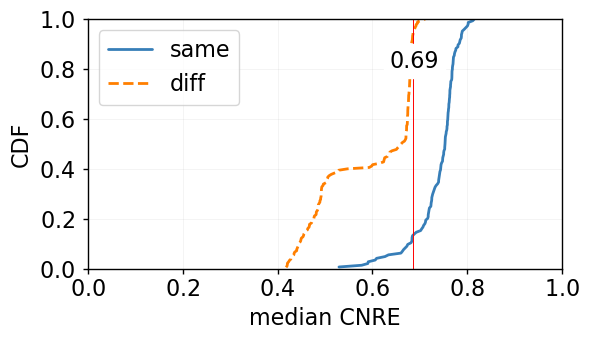
\epsfig{file=figs/cnre_vs_category/country.png, width=1\linewidth}
                \caption{country} 
                \label{fig:vscountry}
            \end{subfigure}
            \begin{subfigure}[b]{0.33\linewidth}
                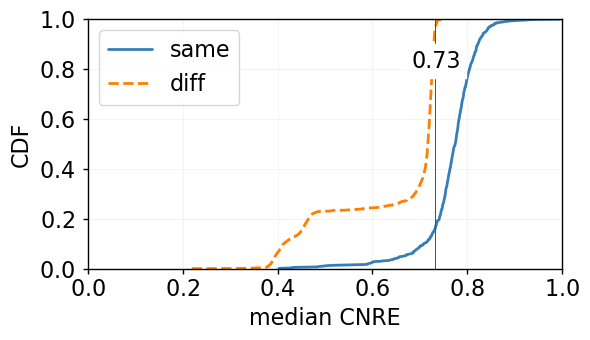
\epsfig{file=figs/cnre_vs_category/asn.png, width=1\linewidth}
                \caption{ASN} 
                \label{fig:vsasn}
            \end{subfigure}
            \begin{subfigure}[b]{0.33\linewidth}
                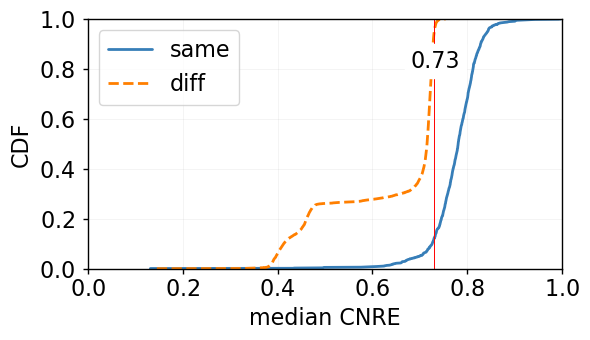
\epsfig{file=figs/cnre_vs_category/prefix.png, width=1\linewidth}
                \caption{BGP prefix} 
            \end{subfigure}
        }
    \caption{CDFs of CNREs across client sets with matching (same) and non-matching (diff) labels. 
    ``Same'' shows the CDF for the median CNRE distance across all client pairs matching a given label. 
    ``Diff'' shows the CDF for the median CNRE distance from each label group
    toward all other labels. The red, vertical line in each subfigure marks the
    95th percentile CNRE for for differing labels.}
    \label{fig:vslabel}

\end{figure*}

We compare established client group labeling schemes  ---
country, ASN, and BGP prefix --- to CNRE similarity between clients with
matching (\emph{e.g.}, same country) and differing (\emph{e.g.}, different
country) labels. Our findings are shown in Figure \ref{fig:vslabel}. The 95th percentile CNRE between groups with differing labels
is marked on each plot by a vertical red line; at this point,
differing and matching labels become distinguishable. For example, in Figure
\ref{fig:vasn}, a pair of clients with CNRE < 0.73 (see 0.27 in
Figure \ref{fig:dendrogram}, which uses CNRE distance) are likely from different
ASes, while clients with CNRE > 0.73 are likely from the AS. Note, however, that
\ref{fig:vslabel} uses \emph{median} values for all points shown. We analyze
this further in \ref{s:labelalgn}. 


Figures \ref{fig:vslabel} and \ref{fig:cnredist} together help provide a possible
explanation for three partiions observed in Figure \ref{fig:dendrogram}. In
Figure \ref{fig:vslabel}, we see that in all three subplots, the aforementioned
middle region of Figure \ref{fig:dendrogram} appears again, this time as a
plateau in both the ``Diff'' and ``Same'' curves. In this region, ``Diff'' and
``Same'' overlap significantly, rendering them indistinguishable. This transient
zone is given further context in Figure \ref{fig:cnredist}, where we shade each
country's median CNRE towards other countries (\emph{i.e.}, outbound
comparisons) --- the same data used to plot the
``Diff'' CDF in Figure \ref{fig:vscountry}. 

If a given country tends to have low CNREs between itself and all other
countries, this implies that the country is exposed to a more exclusive set of
web resources than its peers. For example, Australia, which, as shown in
\ref{fig:vscountry}, has a generally low CNRE with other countries, likely
utilizes very locale-targeted infrastructure given its relative distance from
more more broadly used network resources. Likewise, China, which is well
documented as having its Internet infrastructure deliberately disjoint from much
of the world (CITE great firewall, etc), also has a low CNRE with most other
countries. Conversely, we see most that countries within Europe and Africa tend
toward having higher CNREs with most other countries, implying that the majority
of web resources exposed in those regions are neither exclusive nor fine grained. 

\begin{figure}

    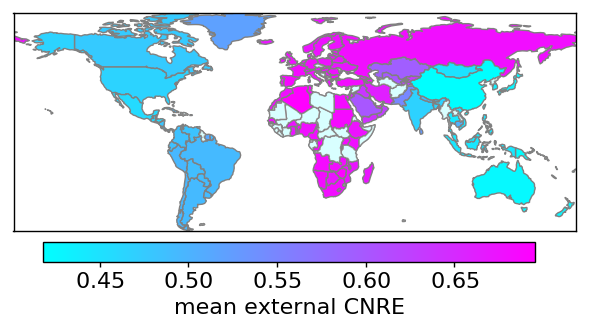
\epsfig{file=figs/cnre_country_uniqueness_map.png, width=1\linewidth}

    \caption{Choropleth with each country shaded by its median CNRE distance
    from all other countries.}
    \label{fig:cnredist}

\end{figure}

\subsection{Label Alignment}
\label{s:labelalgn}

Now that we have established some concept of what constitutes a ``high'' or
``low'' CNRE measure, we further consider CNRE in comparison to country, ASN,
and BGP prefix --- three labeling schemes commonly used group Internet clients.
Specifically, we wish to determine if the information captured by
CNRE (the extent to which clients are exposed to the same web resources) is
reasonably captured by any pre-existing system. If this were the case, one might
argue that the premise of treating CNRE as a separate system would be redundant
and arbitrarily complex. Therefore, we treat this subsection as a means of
validating and justifying the CNRE as a separate, currently unaddressed concept.

In Figure \ref{fig:ch}, we plot the completeness, homogeneity, and number of
clustesr for the aforementioned labeling schemes as we cluster clients in our
dataset, varying the CNRE distance threshold used for cluster formation. In
addition, we also mark, with a vertical line, the CNRE distance at which labels
become distinct (see Figure \ref{s:formation}), and we mark the number of labels
(\emph{i.e.}, the number countries, ASes, or BGP prefixes) present with a
horizontal line (using the righthand y-axis). 

If homogeneity and completeness, which together indicate how well cluster
membership aligns with a given labeling scheme, is not high, the CNRE-related
implications of a given label become ambiguous. We see in Figure \ref{fig:ch}
that for country and ASN, homogeneity and completeness are never simultaneously
high, rendering them unusable for determining CNRE on their own. BGP prefix,
however, requires more thorough consideration. In Figure \ref{fig:chbgp}

\begin{figure*}
    \center
        \mbox{
            \begin{subfigure}[b]{0.33\linewidth}
                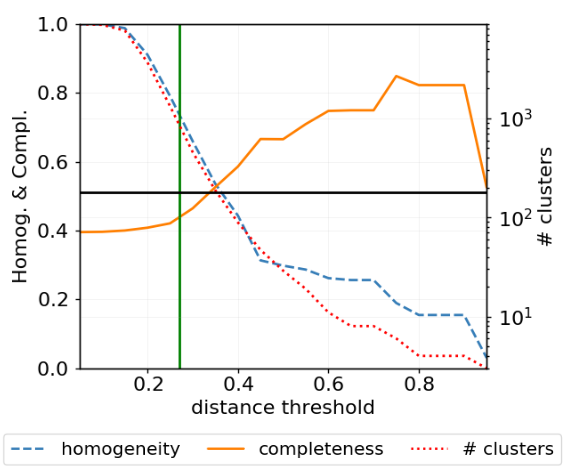
\epsfig{file=figs/completeness_vs_homogeneity/country.png, width=1\linewidth}
                \caption{country} 
            \end{subfigure}
            \begin{subfigure}[b]{0.33\linewidth}
                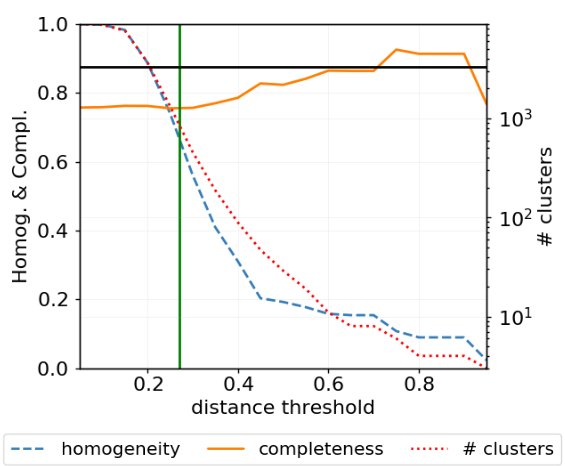
\epsfig{file=figs/completeness_vs_homogeneity/asn.png, width=1\linewidth}
                \caption{ASN} 
            \end{subfigure}
            \begin{subfigure}[b]{0.33\linewidth}
                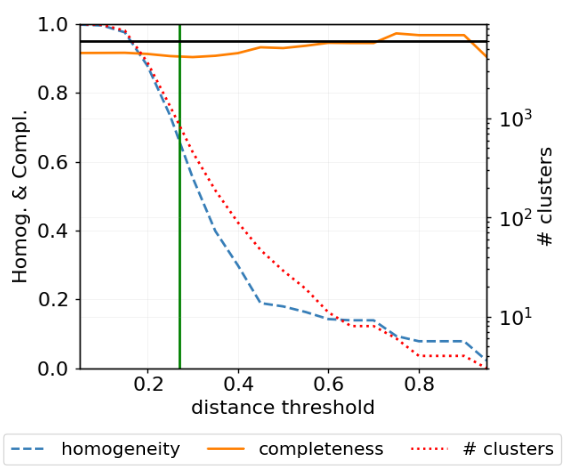
\epsfig{file=figs/completeness_vs_homogeneity/prefix.png, width=1\linewidth}
                \caption{BGP prefix} 
                \label{fig:chbgp}
            \end{subfigure}
        }
    \caption{Completeness, homogeneity, and number of clusters versus clustering
    distance threshold. The vertical line marks 0.27, the CNRE distance at which
    clients with differing labels become distinguishable, and the horizontal
    line denotes (using the right-side y-axis) the number of different real labels
    (for example, the number of countries) preesent in our data set for the
    given labeling scheme.}
    \label{fig:ch}
\end{figure*}


Figure \ref{fig:dendrogram} depicts the hierarchical clustering dendrogram based 
on pairwise CNRE distances.
This representation highlights the similarity of clients and different possible 
partitioning.
Each node in the tree is a cluster composed of the underneath denser clusters.
A horizontal cut in the dendrogram produces a partitioning of clients  for which
the dissimilarity of two probes in the same partition is not greater than the 
y-value where the cut is done. 

For example, the colored clusters in Figure~\ref{fig:dendrogram} are obtained 
with a cut at $y=0.65$.
This partitioning produces eight clusters including three small ones 
composed of outliers.
The five large clusters represent a very coarse partitioning of clients.
95\% of probes in the green cluster are from Europe and 4\% are from Africa 
(that is almost all African probes), the red cluster consists mainly of
German, Italian, and Russian probes (79\%), the blue cluster is mainly North and
South American probes (resp. 80\% and 18\%), the khaki cluster has mostly probes
from Asia and Oceania (resp. 67\% and 32\%), and the black cluster is mostly
North American probes (98\%).
As each cluster is composed of smaller and denser clusters, one can again partition
these clusters and form groups with clients having more network resources in common.

    \section{Cluster Analysis} \label{sect:analysis}

Now that we have built up an understanding of how CNRE behaves, we move on to
investigate the aggregate catchments of clients using clustering techniques
discussed in the previous section. In this section, we use the aforementioned
CNRE threshold of 0.73 for cluster formation. This threshold yields 870
clusters.  For analysis, in which we compare clients that cohabit the same
cluster, we consider only clusters for which the dataset has a representation of
at least three clients; this yields 612 clusters from the original 870. The
average cluster size from this reduced set is 15.78 members, with a standard
deviation of 9.0 and a median size of 14.19. Note that cluster size variety is
significantly impacted by the dataset, which has more client representation
in western Europe and North America than in the rest of the world where RIPE's
influence is more sparse \cite{ripe-atlas}.


Here we examine each cluster's geographic spread --- the closeness, in terms of
geographic distance, of members of the same cluster. As clients sharing the same
cluster are predominantly exposed to the same network resources, the geographic
spread of a cluster's clients must related to the network performance (latency)
they experience. Specifically, if a pair of clients directed
to the same network resource are physically ``far'' apart from each other, it is
likewise impossible for \emph{both} clients to simultaneously be near said
resource. In such an arrangement, the resource is either near one client and far from the other, or the
resource is equidistant from both clients. In the latter case, if the clients
are sufficiently far from each other, the resource must also be far from both clients.

To calculate these geographic distances, we use coordinates for RIPE Atlas
probes --- our client machines in the context of this experiment --- obtained
from RIPE Atlas's API. RIPE acquires probe location information via manual input
from volunteers who themselves maintain Atlas probes, and, where necessary, by
autmated input from MaxMind \cite{maxmind}. Figure \ref{geomeans} shows the CDF of the
mean geographic distance (in kilometers) between members of a cluster, for each
cluster. Members of a cluster with a larger mean geographic distance are farther
apart from each other, on average, than are the members of a cluster with a
lower mean geographic distance. In the median case, we see an average client
distance of 509 km. We observe that for 20\% of clusters, members are over 1000
km on average.  


\begin{figure}
    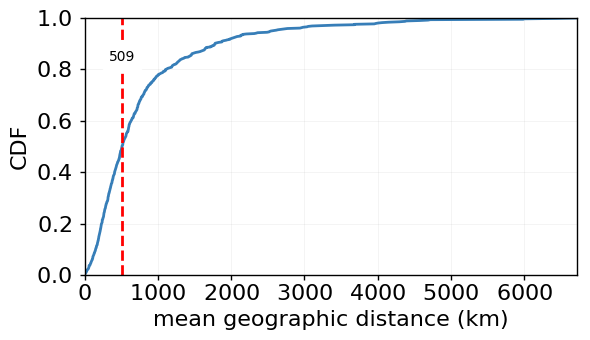
\epsfig{file=figs/geo_means.png, width=1\linewidth}
    \caption{CDF of mean geographic distance between
    cluster members. The dashed vertical line marks the median.}
    \label{geomeans}
\end{figure}

Since CNRE potentially spans many, physically distinct resources, it serves as
an \emph{aggregate} measurement, and we do not attempt to pinpoint the location
of any individual resource. Instead, we identify the effective ``center'' of
each cluster and measure the effect of a member's distance from the center.
Figure \ref{centerlocs} marks a point for the the coordinates of each cluster's
center. The disproportionately high number of centers located in Europe is
byproduct of the distribution of RIPE Atlas probes, which are most densely
concentrated in Europe where RIPE operates. 

\begin{figure*}
    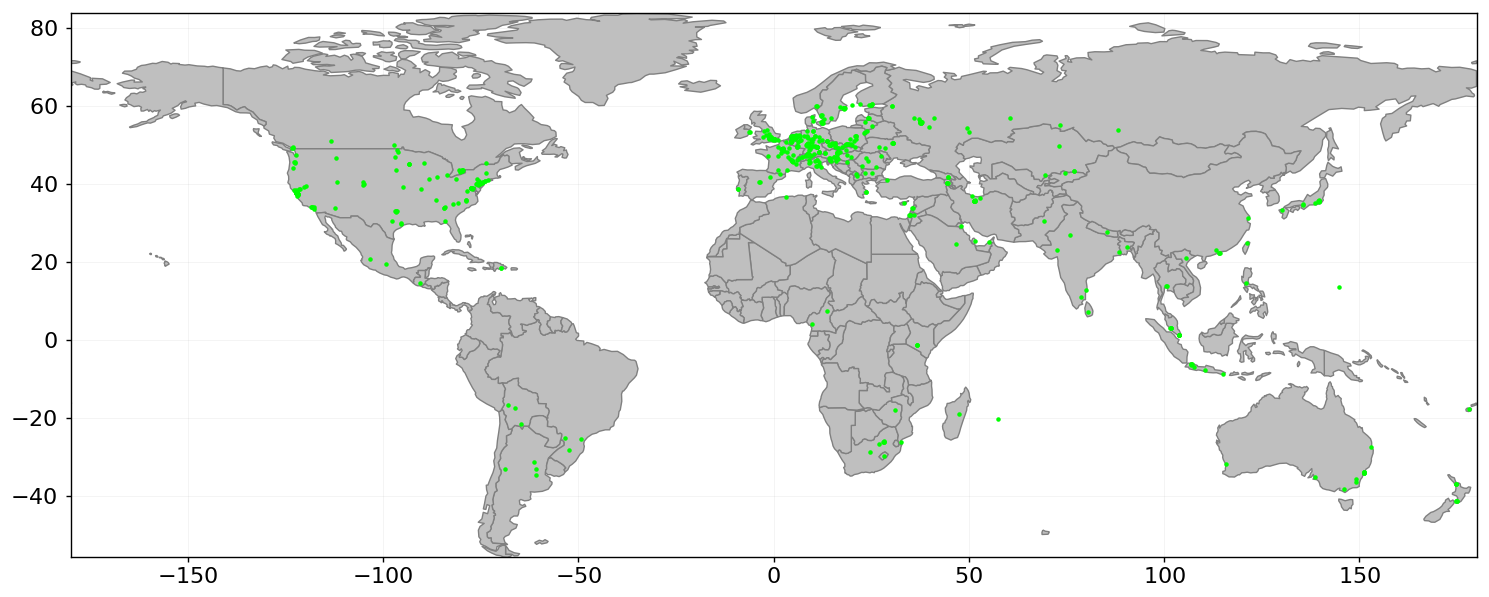
\epsfig{file=figs/geo_centers.png, width=1\linewidth}
    \caption{Map of world with point for each cluster's geographic center.}
    \label{centerlocs}
\end{figure*}


Following the intuition of DNS redirection laid out in other work
\cite{Calder2013,exploringedns,benchaita2016stability}, we hypothesize that the
geographic center of a cluster will sit physically close the location of the
most of that cluster's network resources. By this logic, clients closer to
their cluster's center should experience better network performance
(\emph{i.e.}, lower latency) than those farther away. To test this, we compared
each client's mean latency (taken across all 299 ping responsive domains in our
set) to that client's distance from its respective cluster's center. For
simplicity, we use a cluster's geometric median as an estimate of its center.
The results of this comparison are shown in Figure \ref{geoperf} as a scatter
plot of mean latency versus distance from cluster center. Each point
corresponds to a single client's latency and distance from its respective
cluster's center.  The figure also includes a best fit line, denoting the
overall trend of the points. 

Note the positive slope of points in Figure \ref{geoperf}, indicative of a
directly proportional relationship between latency and distance from the
cluster's effective center. As a client's distance from its cluster's center
increases, so does its latency. Performance for clients relatively near their
respective centers --- closer than 1000 km --- is seemingly noisy and no trend
is clearly observable.  However, as the geographic distance increases beyond
1000 km, the directly proportional relationship between performance and center
distance becomes more apparent. 

\begin{figure}
    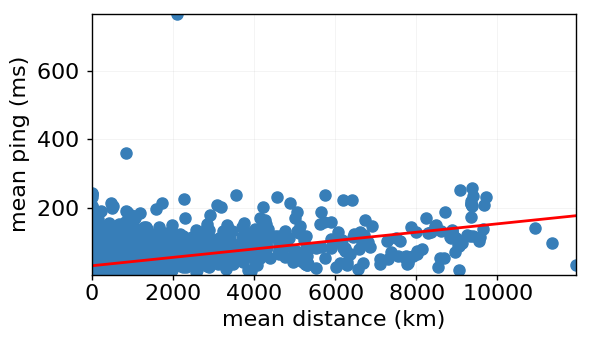
\epsfig{file=figs/geo_vs_perf.png, width=1\linewidth}
    \caption{Scatter plot where, for each client, we compare the client's mean latency
    (across all responding sites) to that client's distance from its cluster's
    center. The line denotes a first order best fit curve for the scatter plot's points.}
    \label{geoperf}
\end{figure}

Also note that the slope of Figure \ref{geoperf}'s best fit line
quantifies this relationship as approximately
$8.2\times10^{7}$m/s, which implies a general data speed of
approximately one half of the speed of light. This is comparable to the transmission speeds of the fastest network communication mediums in use at the
time of this writing --- approximately $\frac{2}{3}$rds of the speed of
light \cite{gueye2006constraint,speedoflight}. Traffic, routing complexity, and the pressence of lower speed
mediums or hops (\emph{i.e.}, bottlenecks) may account for the apparently lower speed in our finding.


\begin{figure}
        \begin{subfigure}[b]{0.8\linewidth}
            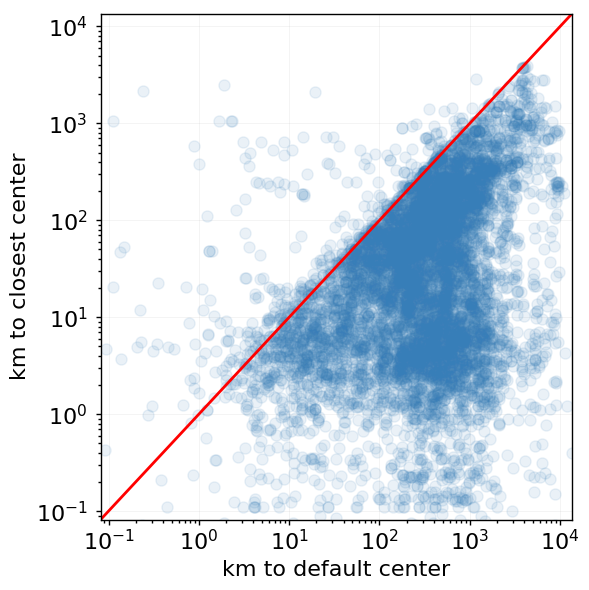
\epsfig{file=figs/nearest_centers_dist.png, width=1\linewidth}
            \caption{geographic distance}
            \label{nearest_center_dist}
        \end{subfigure}
        \begin{subfigure}[b]{0.8\linewidth}
            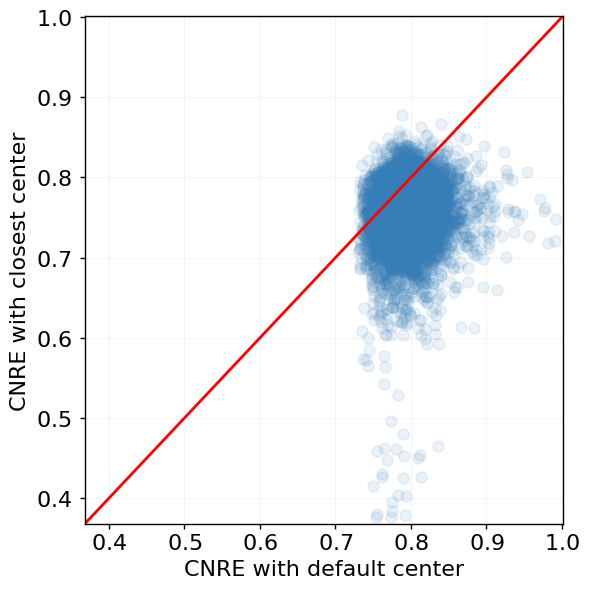
\epsfig{file=figs/nearest_centers_cnre.png, width=1\linewidth}
            \caption{CNRE similarity}
            \label{nearest_center_cnre}
        \end{subfigure}
    \caption{Subfigure \ref{nearest_center_dist} shows a scatter plot of each client's geographic distance from its own
    (``default'') cluster's
    center location versus its geographic distance to the geographically closest center of
    another cluster (``closest'').
    Subfigure \ref{nearest_center_cnre} shows a scatter plot of each client's CNRE similarity with its own
    (``default'') cluster's
    center location versus its CNRE similarity with the geographically
    closest center of
    another cluster (``closest'').}
    \label{nearest_centers}
\end{figure}

As we have demonstrated that one's distance from their cluster's center impacts
performance, clients should ideally share resources with the closest cluster
center possible. Figure \ref{geoperf} raises an additional concern: many clients
are very far away --- often thousdands of kilometers --- from their respective
cluster centers.  For perspective, we remind the reader that the circumference of
the world is approximately 40,075 km; several clients reside over a fourth of
that distance from their cluster's center. With such large geographic distances,
however, it is likely the case that there exists some \emph{alternative} cluster
whose center is geographically nearer to the client than the client's own
cluster's center. For clarity, we will refer to a client's own cluster's center
as its ``default'' center, and the cluster center geographically closest to the
client (excluding the ``default'' center) as the ``closest center'' or
``alternative center''. In Figure \ref{nearest_centers}, we compare the
properties of each client's default and closest centers.

Subfigure \ref{nearest_center_dist} shows a scatter plot of the geographic
distance from each client (in kilometers) to its default and closest centers.
The diagonal line dividing the plot indicates where the geographic distances are
equal.  Points beneath the line correspond to clients who are closer to their
alternative centers, while clients with points above the line are closest to
their default centers. Most clients are closer to their alternative centers, but
there are several details to note, discussed below. 

First, it is apparent that most clients are geograhpically closer to their
alternative cluster centers than their default centers, in some cases by orders
of magnitude. Second, we remind the reader that we employed the complete linkage
method to form our hierarchical clusters. Because of the behavior of complete
linkage, which determines cluster membership by pairwise distance across all
members instead of individual members, it is possible that individual clients
may have a higher CNRE similarity with their alternative center than with their
default center. In other words, it may be the case that we have assigned some
clients to the ``wrong'' cluster. Occurrances of this may account for some of
the noise observed in default center distances below 1000 km in Figure
\ref{geoperf}. To test for mismatched clients, we plot a point for each client's CNRE similarity
towards its closest center versus its default center in Subfigure
\ref{nearest_center_cnre}. The majority of CNRE
values in Subfigure \ref{nearest_center_cnre} are concentrated between 0.7 and
0.8. This suggests that geograhpically overlapping resource allocation groups
may be responsible for the behavior observed in the ambiguous regions of Figures
\ref{fig:dendrogram} and \ref{fig:vslabel}. 

Although 95.18\% of clients had alternative centers geographically closer than
their default centers (274.69 kilometers closer in the median case), 16.48\% of
these geographically closer 
clients had higher CNRE similarity with their default centers (1.99\% higher in
the median case). While we have demonstrated that high geographic distance
coupled with high CNRE tends to result in higher latency, here we paradoxically
observe that this arrangement is a common occurence. We further explore the
implications of this pattern in Section \ref{discussion}.


    \section{Discussion} \label{discussion}
\subsection{Why Web Object Domains}

In Section \ref{domcollect}, we described how the set of domains used in my
experiment were selected. The selected domains were extracted directly
from web object URLs observed across the set of checked web pages. Note
that these domains are often abstractions of more explicit hosting schemes.
For example, such domains may resolve to unique CNAMES or directly resolve
to third party CDN addresses \cite{Su2006}. In contrast to my approach, we could have
converted each domain into some lower level representation (such as its CDN) and
in turn performed a CNRE-like measurement study using this representation
(\emph{i.e.}, ping from each client to each CDN in the set).

While this alternative approach may provide its own insights, we chose leave
each discovered domain ``as is'' for two reasons. First, although a given domain
may use CDN hosting, it is worth noting that modern CDN selection techniques are
complex and diverse. While some content providers may opt to utilize a
\emph{single} CDN for their purposes, it has also become common practice to
instead depend on CDN \emph{brokers} or \emph{multi} CDNs to dynamically (by
cost, performance, geography, \emph{etc.}) make use of a set of CDNs. In other
words, the ``less abstract'' representation of a given content provider is, in
many cases, far from comprehensive with regard to a diverse set of clients.
Second, even if a domain or content provider could adequately be reduced to a
lower level description as described, the performance of a given CDN ``in
general'' is not necessarily representative of the performance of one of its
customers. The reasons for this are plentiful, ranging from customer specific
policies and agreements (for example, the customer might purchase region
specific support) to caching algorithms and load balancing. 


    \section{Summary}

In this paper, we performed a large scale analysis of cross-domain DNS
redirection for 9,024 globally distributed clients. Our experiments spanned 
302 content hosting domains, shown to often coexist within the same popular web pages.
To quantify our findings, we introduced common network resource exposure, a
similarity measure that captures the extent to which clients are directed to the
same content resources. We validated CNRE as a necessary new measure by formally demonstrating that existing alternative labeling schemes fail to adequately
capture the same information.

Having established CNRE, we investigated the properties of high and low CNRE
measures between clients, and, from our findings, we derive CNRE \emph{clusters},
representative of aggregate content resource catchments. Finally, we have shown that a
client's geogrpahic relationship with its cluster's center is directly
proportional to that client's average performance across hundreds of domains. In
summary, our work in this project provides a baseline by which we can better
understand content resource allocation patterns, independent of the case specific
concerns of individual hosting implementations.

%   ==========================================================================
%   Wrap up the document with the Bibliography (looks for the specified .bib)
%   ==========================================================================
    \clearpage

    \bibliographystyle{ACM-Reference-Format}
    %\bibliography{skylines} 
    \bibliography{bibliography} 
\end{document}
